\documentclass[12pt]{article}

\usepackage[margin=1in]{geometry}
	%changes default margins

\usepackage{setspace}
\doublespacing
	%\singlespacing,\onehalfspacing,\doublespacing can be set and everything thereafter will use that spacing. You can switch within the document as often as you wish
	
\usepackage{parskip}
%changes paragraphs to have an extra space and new indentation with paragraphs, rather than indenting every new paragraph. This is completely a stylistic choice and neither is better than the other.


\usepackage{mathtools,amssymb} %useful math stuff. there are a lot of ams* packages. If you have a math need, it's probably in there

	
	
%\usepackage{natbib}
%\usepackage{biblatex} %natbib is older and available from almost all journals, biblatex is not, but biblatex has more flexibility and options.

%\usepackage[natbib=true]{biblatex} %this often works and requires minimal changes 

%for biblatex you write \textcite{citekey} and \parencite{citekey}
%for natbib you write \citet{citekey} and \citep{citekey}. Please avoid using \cite{} since you won't control whether it's parenthetical, but you are responsible for whether you use something in text or parenthetically.
%for \usepackage[natbib=true]{biblatex} you follow the natbib style and you won't have to perform search/replaces in your document, you would only need to change the package call and bibliography call.

\usepackage{natbib}
\bibliographystyle{chicago}

%other useful packages
% \usepackage{graphicx} %for including images including pdf



\title{As1: The Three-Body Problem}
\author{cijsp}
\date{\today}

\begin{document}
	
	\maketitle
	
	\section{Introduction}

This report presents an analysis of residuals in Simple Linear Regression, utilizing Anscombe's Quartet dataset. The parameters of the linear model is determined through maximum likelihood first, the residuals of each dataset is then analyzed. Through this analysis, our objective is to enhance our comprehension of possible challenges and limitations inherent in the execution of linear regression.
	
	\section{Data Description}
	
Anscombe's Quartet is a dataset constructed in 1973 by the statistician Francis Anscombe \citep{Anscombe1973}. It serves as a compelling illustration of the critical role that data visualization plays in analysis. This dataset emphasizes the impact of outliers and influential observations on statistical characteristics, underscoring the limitations of relying solely on summary statistics without considering the underlying data distribution.

The scatter plot in Figure~\ref{Fig:anscombe} illustrates datasets 1 through 4 with their respective fitted lines. Each dataset consists of $n=11$ data points, resulting in identical sample summary statistics, including the mean values of $x$ ($\overline{x} = 9.00$) and $y$ ($\overline{y} = 7.50$), the variances of $x$ ($\text{Var}(x) = 11.0$) and $y$ ($\text{Var}(y) = 4.1$), as well as the covariance of $x$ and $y$ ($\text{Cov}\left(x,y\right)=5.5$). Despite these consistent statistical measures, the scatter plots exhibit distinct visual patterns, highlighting the nuanced differences inherent in each dataset.

\begin{figure}[htbp]
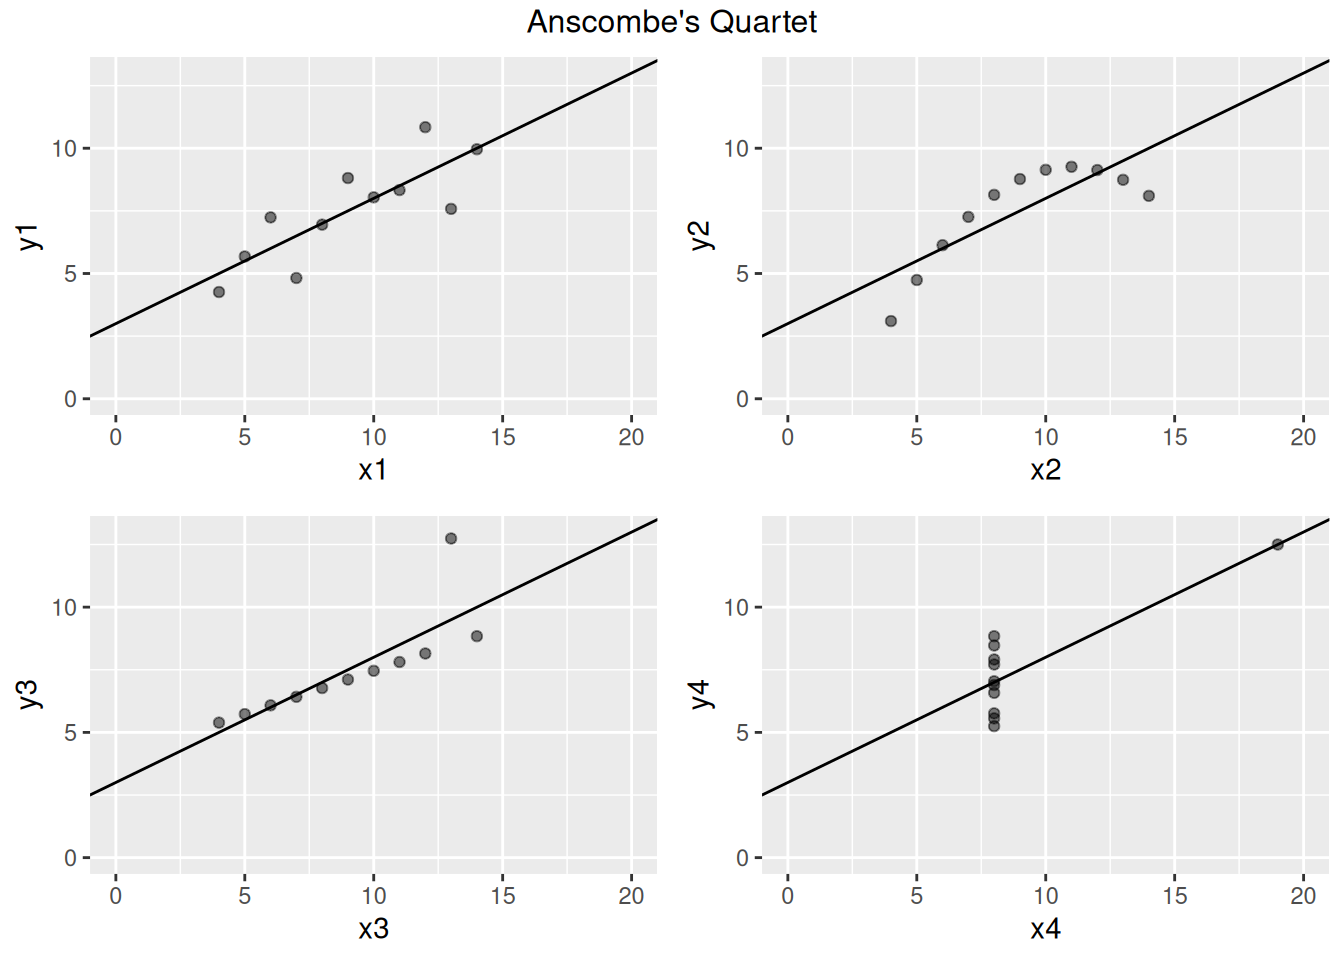
\includegraphics[width=.7\textwidth]{anscombe.png}
\centering
\caption{A Comparative Visualization of Anscombe's Quartet: Scatter Plots and Fitted Lines for Datasets 1--4.}
\label{Fig:anscombe}
\end{figure}


	\section{Simple Linear Regression}

%Let $S_{xx} = \sum\left( x_{i} - \overline{x} \right) ^2$, and let $\tilde{\mu_i} = \tilde{b_{0}} + \tilde{b_1}x_i$ be the estimator for the fitted value for the linear model $\mathbf{y = X b}$.
%
%We have $V\left( \tilde{\mu_i} \right)  = \sigma^2 \left( \frac{1}{n}+\frac{\left( x_i - \overline{x} \right) ^2}{S_{xx}} \right) $

%	We use linear model 
%	$\hat{\mathbf{y}} = \mathbf{X}\hat{\mathbf{b}}$  
%	to fit the four groups of data, where 
%	$\hat{\mathbf{b}} = (\mathbf{X}^T\mathbf{X})^{-1}\mathbf{X}^T\mathbf{y}$,
%	and $\mathbf{X} = [\mathbf{1}, \mathbf{x}]$, $\mathbf{x}$ is the regressor of each group of data. 
%	Rewriting $\hat{\mathbf{b}}$ in scalar form: 
%	$\hat{\mathbf{b}} = \left( b_0,b_1 \right)^T $,
%	where $b_1 = \frac{S_{xy}}{S_{xx}} = \frac{\text{Cov}(\mathbf{x},\mathbf{y})}{\text{V}(\mathbf{x})}$ 
%	and $b_0 = \overline{y} - b_1 \overline{x}$. 
%	The coefficient of determination $R^2 =1-\frac{\text{SSR}}{\text{SST}} = 1 - \frac{\rVert \mathbf{y} - \hat{\mathbf{y}}\rVert^2}{\rVert \mathbf{y} - \overline{y}\cdot\mathbf{1}\rVert^2} $.
%	The calculation results are shown in Table~\ref{tab:1}.

We employ a simple linear model, denoted as $\hat{\mathbf{y}} = \mathbf{X}\hat{\mathbf{b}}$, to fit the four distinct datasets. Here, the parameter vector $\hat{\mathbf{b}}$ is determined using the formula $\hat{\mathbf{b}} = (\mathbf{X}^T\mathbf{X})^{-1}\mathbf{X}^T\mathbf{y}$, with $\mathbf{X} = [\mathbf{1}, \mathbf{x}]$ and $\mathbf{x}$ representing the regressor for each dataset. Expressing $\hat{\mathbf{b}}$ in scalar form as $\hat{\mathbf{b}} = \left( b_0,b_1 \right)^T$, we know that $b_1 = \frac{S_{xy}}{S_{xx}} = \frac{\text{Cov}(\mathbf{x},\mathbf{y})}{\text{Var}(\mathbf{x})}$ and $b_0 = \overline{y} - b_1 \overline{x}$. The coefficient of determination is computed as $R^2 = 1-\frac{\text{SSR}}{\text{SST}} = 1 - \frac{\rVert \mathbf{y} - \hat{\mathbf{y}}\rVert^2}{\rVert \mathbf{y} - \overline{y}\cdot\mathbf{1}\rVert^2}$. 

Detailed calculation results are available in Table~\ref{tab:1}. Notably, all four models yield identical parameters and $R^2$ values. This observation is not surprising, given that the mean, variance, and covariance of both $x$ and $y$ across each dataset are the same.

	\begin{table}[htpb]
		\centering
		\begin{tabular}{|c|c|c|c|c|}
			\hline
			 & 1 & 2 & 3 & 4  \\
			\hline
			$b_0$ & 3.00 & 3.00 & 3.00 & 3.00  \\
			\hline
			$b_1$ & 0.50 & 0.50 & 0.50 & 0.50  \\
			\hline
			$R^2$ & 0.67 & 0.67 & 0.67 & 0.67  \\
			\hline

		\end{tabular}
		\caption{Simple Linear Regression model parameters $b_0, b_1$ and the coefficient of determination $R^2$ for Datasets 1--4.}
		\label{tab:1}
	\end{table}


%	$S_{xx} = \sum \left( x_i - \overline{x} \right)^2 $,
%	$S_{xy} = \sum \left( x_i - \overline{x} \right)\left( y_i - \overline{y} \right) $

	
	\section{Residuals Analysis}
	
%	In this section, we focused on the residuals. The mean of residuals are 0 for all four datasets; The variance of residuals are 1.37 for all four datasets; Figure~\ref{Fig:QQplot} gives the Q-Q plots of each dataset. It is used to examine if the residuals are normal distributed. Ideally, they should fall into the diagnal red line. However, we can see that residuals from dataset 2 are heavy-tailed and the residuals from dataset 3 are right-skewed. This can also be observed in Figure~\ref{Fig:Histogram}.
		
In this section, our emphasis lies on the examination of residuals. Notably, the mean of residuals is 0 across all four datasets, while the variance remains around 1.37. Figure~\ref{Fig:QQplot} presents Q-Q plots for each dataset, serving as a tool to assess the normal distribution of residuals. Ideally, these points should align along the diagonal red line. However, it is evident that residuals from dataset 2 exhibit a heavy-tailed distribution, and those from dataset 3 demonstrate a right-skewed pattern, as further illustrated in Figure~\ref{Fig:Histogram}.

\begin{figure}[htbp]
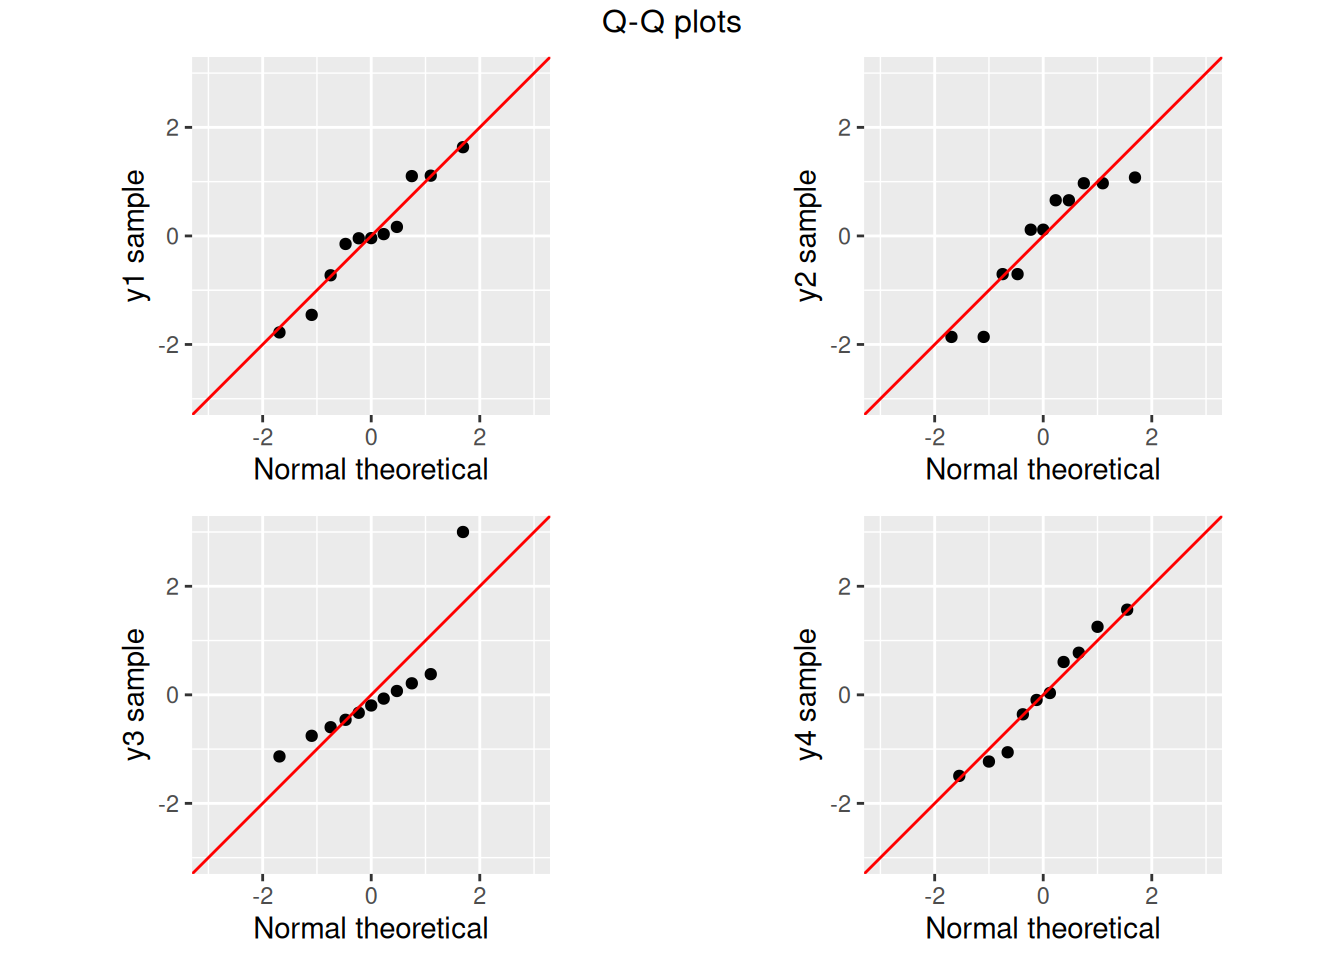
\includegraphics[width=.8\textwidth]{QQplot.png}
\centering
\caption{Q-Q Plots for Residuals: Comparison of Normal Distribution Fit Across Datasets.}
\label{Fig:QQplot}
\end{figure}

\begin{figure}[htbp]
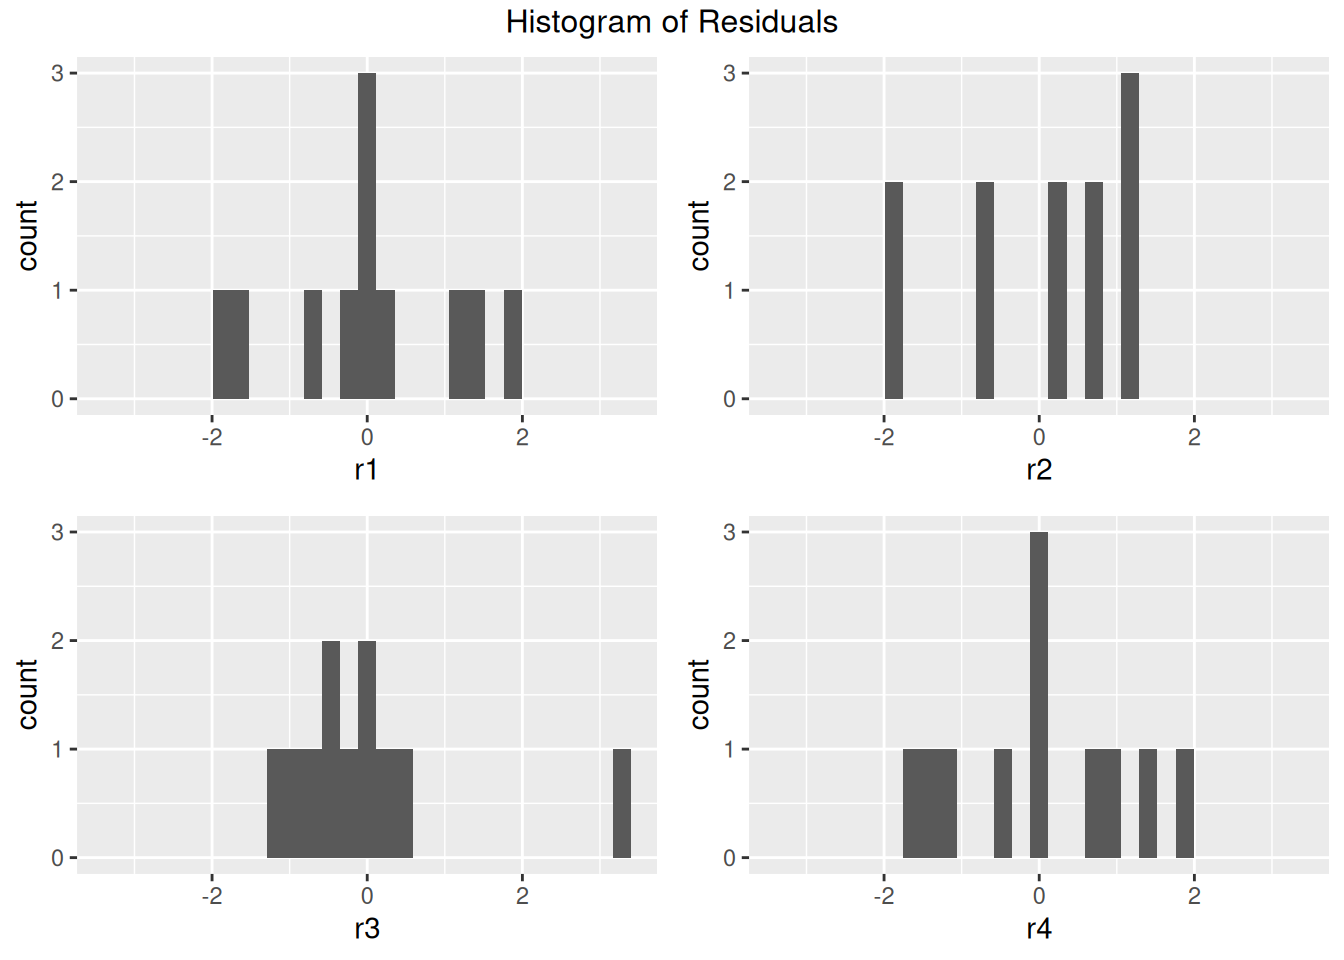
\includegraphics[width=.7\textwidth]{histogram.png}
\centering
\caption{Histograms of Residuals}
\label{Fig:Histogram}
\end{figure}

\newpage
The Residuals vs Fitted Values plot (Figure~\ref{Fig:RVF}) serves as a diagnostic tool for assessing the linearity of the relationship between $x$ and $y$. An ideal scenario is characterized by residuals being evenly dispersed around the fitted values of $y$, akin to the pattern observed in Dataset 1. Deviations from this pattern, such as diminishing (or amplifying) residuals with increasing $y$ (as seen in Dataset 3) or the presence of a quadratic curve pattern as $y$ increases (as evident in Dataset 2), may indicate a non-linear association between $x$ and $y$.
%The Residuals vs Fitted values plot demonstrates whether there is a linear relationship between $x$ and $y$. Ideally, we would like to see that the residuals are evenly distributed across the fitted value of $y$ (like Dataset 1). If residuals become smaller (or larger) as $y$ increases (like Dataset 3), or if residuals shows quadratic curve pattern as $y$ increases (Dataset 2), it might indicate a non-linear relationship between $x$ and $y$.

\begin{figure}[htbp]
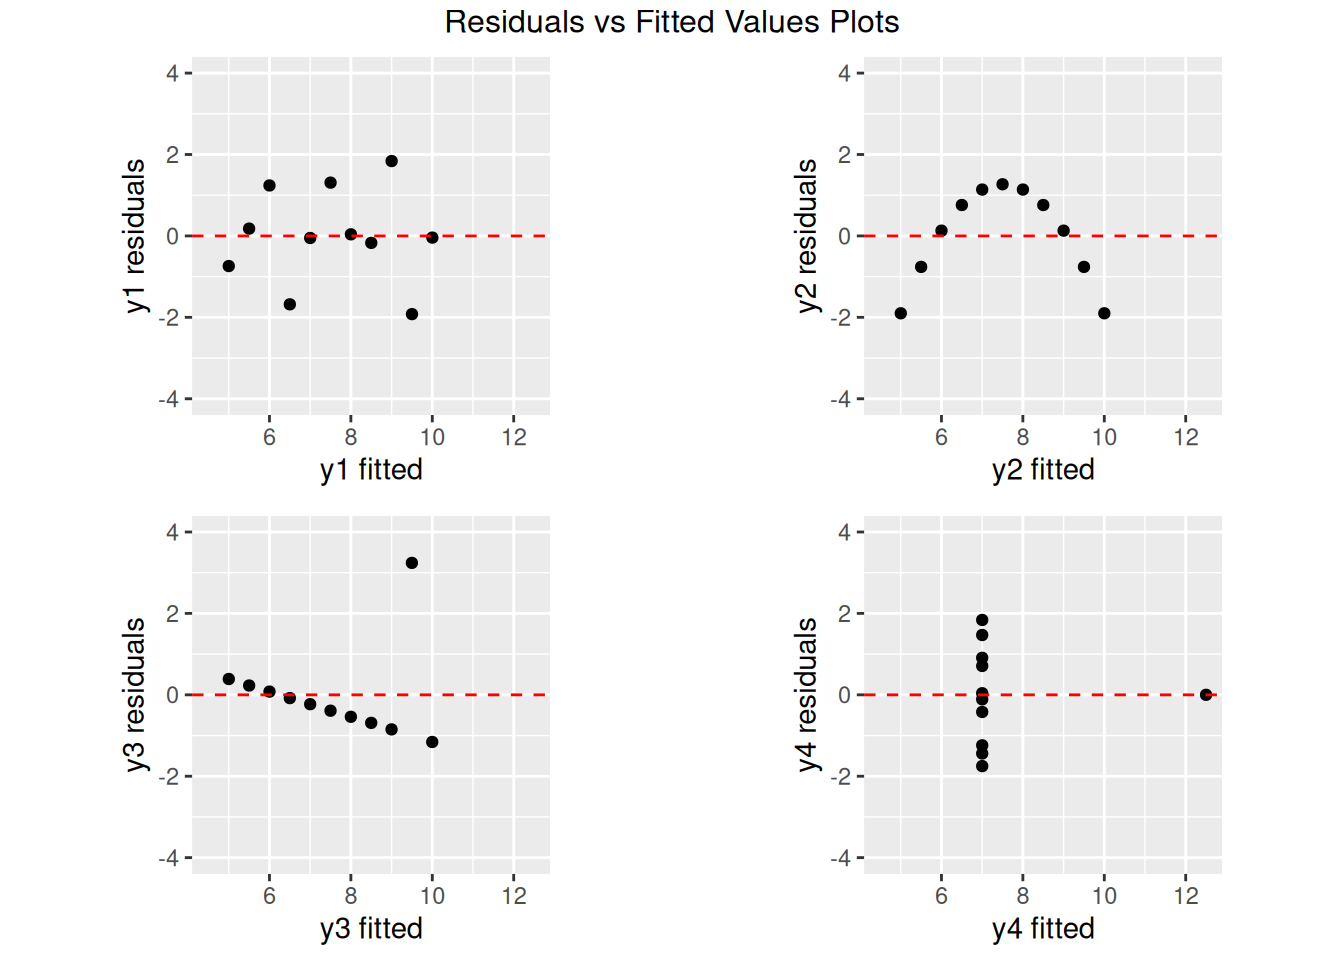
\includegraphics[width=.7\textwidth]{RVF.png}
\centering
\caption{Residuals vs Fitted values}
\label{Fig:RVF}
\end{figure}

The Residuals vs Leverage plot (Figure \ref{Fig:RVL}) illustrates the impact of extreme data points. While both Datasets 3 and 4 contain outliers, it is noteworthy that the outlier in Dataset 4 exerts the most significant leverage on our fitted model.

\begin{figure}[htbp]
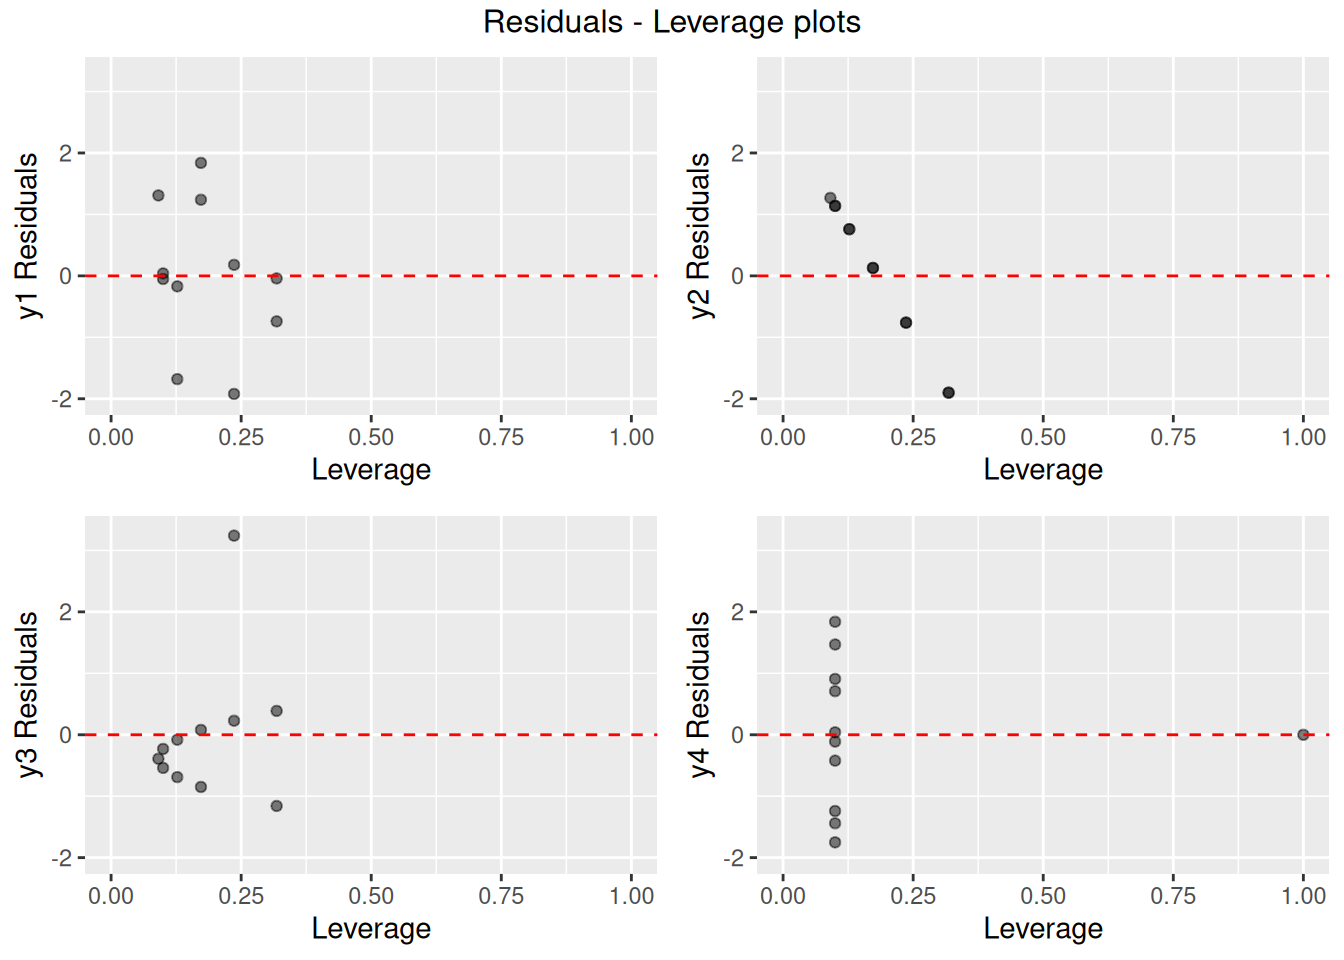
\includegraphics[width=.7\textwidth]{RVL.png}
\centering
\caption{Residuals vs Leverage plots}
\label{Fig:RVL}
\end{figure}

\bibliography{cite}

	
\end{document}

